\section{Überblick}
\subsection{Motivation}
Zur Anwendung von formalen Sprachen in der Informatik gehören unter anderem Scanner und Parser\cite{Aho86}. 
Programmgeneratoren, welche z.B. Parser generieren existieren bereits für Sprachen wie \textsc{Java}\cite{javacup:2016}, \textsc{C}\cite{donnelly1990} usw.
In der Vorlesung "Formal Languages and their Applications"\cite{stroetmann:formallanguages} werden momentan verschiedene Tools genutzt um Parser zu generieren. Dazu gehören u.a. \textsc{JavaCup} zum Erstellen von LALR-Parsern, sowie \textsc{ANTLR4}\cite{parr:2012} für die Erstellung eines Top-Down-Parsers mit Nutzung von EBNF-Grammatiken.
Ziel dieser Studienarbeit ist es eine Alternative zur Nutzung von \textsc{JavaCup} zu ermöglichen. Dies soll geschehen, indem ein Parser-Generator in der Programmierprache \textsc{SetlX} geschrieben wird. \textsc{SetlX} ist eine mengenbasierte Programmiersprache. Sie kann mit dem \textsc{SetlX}-Interpreter genutzt werden. Dieser ist unter der folgenden Adresse verfügbar:\\
\href{http://randoom.org/Software/SetlX}{{http://randoom.org/Software/SetlX}}\\
Diese Programmiersprache wird in den Vorlesungen der theoretischen Informatik\cite{stroetmann:logic}\cite{stroetmann:algorithms} bereits ausgiebig genutzt. Eine Ergänzung für die Vorlesung über die formalen Sprachen kann somit den Studenten helfen die Konzepte des Parsens zu verstehen, ohne in eine andere Programmiersprache "umzudenken". Da der Parser-Generator sehr stark an \textsc{JavaCup} orientiert ist, entstand der Name \textsc{SetlCup}. Ein großer Unterschied ist jedoch, dass \textsc{SetlCup} ein LR-Parser-Generator ist.

%\textsc{SetlCup} ist ein Programmgenerator, d.h. er nimmt die Beschreibung einer Sprache als Eingabe und produziert ein \textsc{SetlX} Programm, welches als Scanner und Parser agiert. Genauer genommen ist \textsc{SetlCup} ein LR-Parser-Generator. Dieser ist angelehnt an \textsc{JavaCup}.
%\begin{enumerate}
	%\item Definition eines Scanners, sowie einer Grammatik für den gewünschten Parser (geschieht durch Nutzer)
	%\item Ausführen von SetlCup zur Generierung des Parsers
	%\item Nutzung des Parsers	
	%\begin{itemize}
		%\item[a)] alleinstehend über die Kommandozeile
		%\item[b)] eingebunden in einen Treiber
	%\end{itemize}
%\end{enumerate}


\section{Funktionalität}
\subsection{Benutzung}
Der Benutzer von \textsc{SetlCup} erstellt durch eine gegebene Scanner- und Parserdefinition eine neue \textsc{SetlX}-Datei. Diese beinhaltet einen kanonischen LR-Parser, welcher auf den gegebenen Definitionen beruht. Anschließend kann eine Eingabedatei von dem generierten Parser überprüft werden. Dabei wird ggf. angegebener Code bei der Reduzierung der entsprechenden Regeln durchgeführt. 
Zunächst wird erklärt, wie die Komponente aufgerufen werden kann.
\section{Aufrufsmethoden}
Es gibt mehrere Möglichkeiten \textsc{SetlCup} aufzurufen:
\subsection{Aufruf über Kommandozeile}
\begin{enumerate}
	\item \begin{Verbatim}
  setlx setlcup.stlx -p parser_scanner_datei
  setlx setlcup.stlx -p examples/math_simple_expression.g
	\end{Verbatim}
			Mit diesem Aufruf wird ein Parser gemäß der in der Eingabedatei gegebenen Definitionen erstellt.
	\item \begin{Verbatim}
  setlx setlcup.stlx -p parser_scanner_datei -d
  setlx setlcup.stlx -p examples/math_simple_expression.g -d
	\end{Verbatim}
			Um die Art und Weise, wie der Parser generiert wird nachvollziehen zu können, kann mit der Option "-d" das Debugging eingeschaltet werden. Dabei wird empfohlen die Ausgabe in eine Datei umzuleiten.
	\item \begin{Verbatim}
  setlx parser_datei -p eingabe_datei
  setlx math_simple_expressionGrammar.stlx -p simple_statement.txt
	\end{Verbatim}
	Der erstellte Parser kann mit dem o.g. Befehl aufgerufen werden und versucht die Eingabedatei nach den angegebenen Regeln zu überprüfen.
		\item \begin{Verbatim}
  setlx parser_datei -p eingabe_datei -d
  setlx math_simple_expressionGrammar.stlx -p simple_statement.txt -d
	\end{Verbatim}
	Analog zur Parsererstellung wird durch die Option "-d" das Debugging eingeschaltet.
	\item \begin{Verbatim}
  setlx setlcup.stlx -p -help
	\end{Verbatim}
			Dieser Aufruf zeigt die Hilfe an, wie \textsc{SetlCup} aufgerufen werden kann.
	\item \begin{Verbatim}
  setlx test_setlcup.stlx
	\end{Verbatim}
			Dieser Aufruf testet die Funktionen des Parsergenerators mit verschiedenen Beispielen.
\end{enumerate}
\subsection{Aufruf in SetlX}
Ein Aufruf von \textsc{SetlCup} ist auch in \textsc{SetlX} selbst möglich. Dazu ist es notwendig die Funktionalität im eigenen Quellcode zu laden:
\begin{Verbatim}
load("setlcup_load.stlx");
generate_parser('examples\math_expression_grammar_ast.g', true);
load('examples\math_expression_grammar_astGrammar.stlx');
result := test_parser_from_file('examples\math_expression_input.txt', true);
\end{Verbatim}
\section{Dateistruktur}
Der Parser-Generator \textsc{SetlCup} ist in mehrere Dateien aufgeteilt.
\paragraph{setlcup.stlx} Diese Datei wird aufgerufen, falls man über die Kommandozeile mit \textsc{SetlCup} arbeiten möchte. Sie nimmt die Definition der Grammatik als Parameter an und gibt sie an die jeweiligen Programme weiter, damit die Generierung des Parsers gestartet werden kann.
\paragraph{setlcup\_load.stlx} Diese Datei lässt zunächst den Scanner und daraufhin den Parser generieren. Falls über \textsc{SetlX} mit \textsc{SetlCup} gearbeitet werden soll, ist es möglich diese Datei als Grundlage zu nutzen. Sie wird u.a. für den Test der Funktionalität benutzt (siehe "test\_setlcup").
\paragraph{scanner\_generator.stlx} In dieser Datei wird die Eingabe analysiert. Es wird der Scanner aus den angegebenen Tokens generiert. Dieser wird daraufhin in einer Ausgabedatei abgelegt. \\
Auch der Parser aus der Datei "\_sr\_parser\_part.stlx" wird der Datei angehangen. Zusätzlich wird die Grammatikdefinition analysiert und  in einer Token-Liste zurückgegeben.
\paragraph{parser\_generator.stlx} Der Parser Generator erstellt den kanonischen LR-Parser. Er erzeugt die notwendigen Action-, State- und Gototabellen. Diese werden zusammen mit den Regeln und dem vom User gewünschten Code auch in der o.g. Datei abgespeichert. 
\paragraph{\_sr\_parser\_part.stlx} Der Shift-Reduce-Parser ist in dieser Datei umgesetzt. Er wird zusammen mit den benötigten Tabellen, sowie dem Scanner in eine neue Datei kopiert. 
\paragraph{\_Grammar.stlx} In dieser Datei wird der erstellte Scanner und Parser abgelegt. Beim Aufruf wird die übergebene Datei geparsed. Dabei werden die o.g. Tabellen, sowie der vorher erstellte Scanner genutzt. Der Parser ist ein Shift-Reduce Parser. Beim Reducen wird der vom User angegebene Code ausgeführt. Der Wert der Variable "result" wird am Ende zurückgegeben.
\paragraph{test\_setlcup.stlx} Für einen Regressionstest kann mit dieser Datei überprüft werden ob alle Beispiele momentan geparsed werden können. Dabei wird für mehrere Grammatiken der Parser erstellt. Diese werden anschließend mit einer Eingabedatei aufgerufen und die Ergebnisse mit den vorher festgelegten verglichen.
\section{Aufbau der Definitionen}

Der Aufbau der Scanner- und Parserdefinitionen ist in drei Abschnitte zu unterteilen:
\begin{enumerate}
	\item Kommentare
	\item Scannerdefinition
	\item Parserdefinition
\end{enumerate}
\subsection{Kommentare}
Im obersten Bereich der Datei ist es möglich die Idee des Parsers zu beschreiben.
Dieser Abschnitt endet mit dem Symbol "`\%\%\%"'. 
\subsection{Scannerdefinition}
Die Aufgabe des Scanners ist es, die Eingabe in eine Liste von Tokens zu zerlegen. Die Syntax\mRefFigure{fig:scanner_def} wird im Folgenden erklärt.
\begin{figure}[!ht]
\begin{Verbatim}[ frame         = lines, 
                  framesep      = 0.3cm, 
                  labelposition = bottomline,
                  numbers       = left,
                  numbersep     = -0.2cm,
                  xleftmargin   = 0.8cm,
                  xrightmargin  = 0.8cm,
                ]
	INTEGER       := 0|[1-9][0-9]*     ;
	ASTERISK      := \*                ;
	WHITESPACE    := [ \t\v\r\s]       ;
	SKIP          := {WHITESPACE} | \n ;
\end{Verbatim}
\caption{Scanner Definition}
\label{fig:scanner_def}
\end{figure}
\begin{enumerate}
	\item In Zeile 1 wird der Token "INTEGER" definiert. Tokens werden auf die folgende Weise deklariert:\\
					token\_name := regex ; \\
					Dabei ist folgendes bei der Syntax des regulären Ausdrucks zu beachten:
					\begin{enumerate}
						\item Die Rückgabe von Capture-Gruppen\footnote{Gruppierungen in regulären Ausdrücken -  \url{https://de.wikipedia.org/wiki/Regulärer_Ausdruck\#Gruppierungen_und_R.C3.BCckw.C3.A4rtsreferenzen}} z.B. "`ab\textbf{(.*)}ab\textbf{(.*)}ab"'	wird konkateniert zurückgegeben (es werden alle einzelnen Unterergebnisse aneinander gehangen).
						\item Die Nutzung der geschweiften Klammer wurde überlagert, sodass die regulären Ausdrücke der großgeschriebene Wörter innerhalb der Klammern im Nachhinein ersetzt werden. Siehe Zeile 4 - "\{WHITESPACE\}".
						\item Ansonsten sind die bereits in \textsc{SetlX} bzw. \textsc{Java} vorhandenen Regex-Ausdrücke benutzbar.
					\end{enumerate}
	\item Wie in \textsc{SetlX} (siehe Zeile 2 und 3) müssen auch in \textsc{SetlCup} vordefinierte Symbole wie $"*","+","?","|","\{","\}","(",")",".","[","]","\backslash"$ escaped werden .
	\item In Zeile 4 wird "SKIP"-Token genutzt. In manchen Fällen werden gewisse Tokens nicht benötigt. Diese können mithilfe des "SKIP"-Tokens ignoriert werden. Dabei ist die Eingabe mit der o.g. Ersetzstrategie ("\{TOKENNAME\}") oder die Nutzung eines regulären Ausdrucks möglich. Verschiedene Tokens müssen mit der Pipe "|" separiert werden.
\end{enumerate}

\subsection{Parserdefinition}
Die Definition der Grammatik für den Parser benutzt Konzepte aus \textsc{JavaCup} und \textsc{ANTLR} \mRefFigure{fig:parser_grammar}.
\begin{figure}[!ht]
\begin{Verbatim}[ frame         = lines, 
                  framesep      = 0.3cm, 
                  labelposition = bottomline,
                  numbers       = left,
                  numbersep     = -0.2cm,
                  xleftmargin   = 0.8cm,
                  xrightmargin  = 0.8cm,
                ]
  grammar         :=  definition_list;
  definition_list :=  rule_definition  definition_list
	              | ;
  rule_definition :=  VARIABLE '::=' body_list ';' ;
  body_list       :=  body '|' neBody_list
	              | body
	              | ;
  neBody_List     :=  body body_list;
  body            :=  element_list action_code;
  action_code     :=  '{:' CODE ':}'
	              | ;
  element_list    :=  element element_list
	              | ;
  element         :=  token;
  token           :=  LITERAL id
	              | TOKEN_NAME id
	              | VARIABLE id ;
  id              :=  ':'VARIABLE
	              |;
  VARIABLE        :=  [a-z][a-zA-Z_0-9]*;
  TOKEN_NAME      :=  [A-Z][A-Z_0-9]*;
  LITERAL         :=  ''[^'']*'';
  CODE            :=  [.\n]*;
\end{Verbatim}
\caption{Grammatik zum Aufbau der Parserdefinition}
\label{fig:parser_grammar}
\end{figure}
\paragraph{VARIABLE} beschreibt den Namen einer Regel z.B. "body". Somit können Regeln referenziert werden.  Außerdem haben auch die IDs einer Variable den gleichen Aufbau. Dies ermöglicht es den Rückgabewert einer Regel bzw. eines regulären Ausdrucks zu nutzen.
\paragraph{TOKEN\_NAME} bezieht sich auf einen Token aus der Scanner Definition.
\paragraph{LITERAL}  beschreibt wortwörtliche Ausdrücke, welche genutzt werden können (z.B. '+', '.', '*', 'print').
	% \begin{enumerate}
	% 	\item Token (defined in the scanner) e.g. "MINUS"
	% 	\item Token in  ' ' e.g. '+' as a literal
	% 	\item other rule\_heads e.g. "prod"
	% \end{enumerate}
	% The Tokens defined in the scanner, as well as the rule\_heads can have an id. This can be used in the action\_code.
\paragraph{CODE} ist ein optionaler Teil einer Regel. Er kann am Ende einer Regel hinzugefügt werden. Der CODE innerhalb der Klammern  wird beim Reduzieren der Regel ausgeführt. Durch die Nutzung der Variable "result" können Ergebnisse zwischen den Regeln transferiert werden. Die IDs der Elemente der jeweiligen Regel können im Code benutzt werden. Der Code selber darf keine Anführungszeichen enthalten. Wenn sie doch notwendig sind, wird empfohlen sie zu escapen mit $\backslash"$ oder den Literalstring z.B. 'a+b = 15' zu nutzen. Außerdem sollte \textbf{generell} auf die Nutzung von Dollarzeichen verzichtet werden. Diese führen zu Komplikationen bei der Serialisierung des Parsers, da sie in \textsc{SetlX} eine Sonderfunktion einnehmen. 
	% \item[|] The pipe separates the different bodies.
\newpage
\section{Beispiele}
Das erste Beispiel beschreibt eine einfache arithmetische Grammatik.
Das zweite Beispiel beschreibt eine simple Programmiersprache.
\subsection{Arithmetische Ausdrücke}
Der arithmetische Parser \mRefFigure{fig:example_arithmetic_grammer} kann mit der oben beschriebenen Syntax definiert werden.
\begin{figure}[!ht]
\begin{Verbatim}[ frame         = lines, 
                  framesep      = 0.3cm, 
                  labelposition = bottomline,
                  numbers       = left,
                  numbersep     = -0.2cm,
                  xleftmargin   = 0.8cm,
                  xrightmargin  = 0.8cm,
                ]
  %%%
  INTEGER       := 0|[1-9][0-9]* ;
  WHITESPACE    := [ \t\v\r\s] ;
  SKIP          := {WHITESPACE} | \n ;
  %%%
  expr 
   ::=  expr:e '+'  prod:p   {: result := print(e+p);  :} 
     |  prod:p               {: result := p;     :}
     ;
  prod 
   ::=  prod:p '*'  fact:f   {: result := p*f; :}
     |  fact:f               {: result := f;     :}
     ;
  fact 
   ::= INTEGER:n             {: result := eval(n); :} 
     ;
\end{Verbatim}
\caption{Parserdefinition für einen simplen arithmetischen Ausdruck}
\label{fig:example_arithmetic_grammer}
\end{figure}
%\lstinputlisting[frame=single,numbers=left,basicstyle=\footnotesize]{math_expression_grammar_ast.g}
Die Generierung des Parsers kann nun über
\begin{Verbatim}
setlx setlcup.stlx -p examples\math_simple_expression.g
\end{Verbatim}
gestartet werden.
Mit einem Treiber Programm\mRefFigure{fig:simple_arith_driver} können eingegebene Ausdrücke geparsed werden.
\begin{figure}[!htb]
\begin{Verbatim}[ frame         = lines, 
                  framesep      = 0.3cm, 
                  labelposition = bottomline,
                  numbers       = left,
                  numbersep     = -0.2cm,
                  xleftmargin   = 0.8cm,
                  xrightmargin  = 0.8cm,
                ]
  load("math_simple_expression_astGrammar.stlx");
  end := false;
  query := "Give an arithmetic Expression: (q for end)";
  while(!end){
    arith_expr :=  read(query);
    if(!("q" in arith_expr)){
      test_parser_from_string(arith_expr, true);
    }
    else{
      end := true;
     }
  }
\end{Verbatim}
\caption{Beispiel für Treiber}
\label{fig:simple_arith_driver}
\end{figure}
Der Treiber kann mit dem folgenden Kommando aufgerufen werden:
\begin{Verbatim}
setlx math_simple_expression_driver.stlx
\end{Verbatim}
Beispielausgabe:
\begin{Verbatim}
Give an arithmetic Expression: (q for end)4*5+3*6
38
Give an arithmetic Expression: (q for end)3+6*4*5
123
\end{Verbatim}
%Eine beispielhafte Eingabe besteht aus drei verschiedenen mathematischen Termen \ref{fig:example_arithmetic_input}.
%\begin{figure}[!ht]
%\begin{Verbatim}[ frame         = lines, 
                  %framesep      = 0.3cm, 
                  %labelposition = bottomline,
                  %numbers       = left,
                  %numbersep     = -0.2cm,
                  %xleftmargin   = 0.8cm,
                  %xrightmargin  = 0.8cm,
                %]
%\end{Verbatim}
%\caption{Beispiel für arithmetische Terme}
%\label{fig:example_arithmetic_input}
%\end{figure}
%Die Ausgabe des AST\mRefFigure{fig:arith_expr_tree} beschreibt die gezeigte Eingabe.
%\begin{figure}[!ht]
	%\centering
		%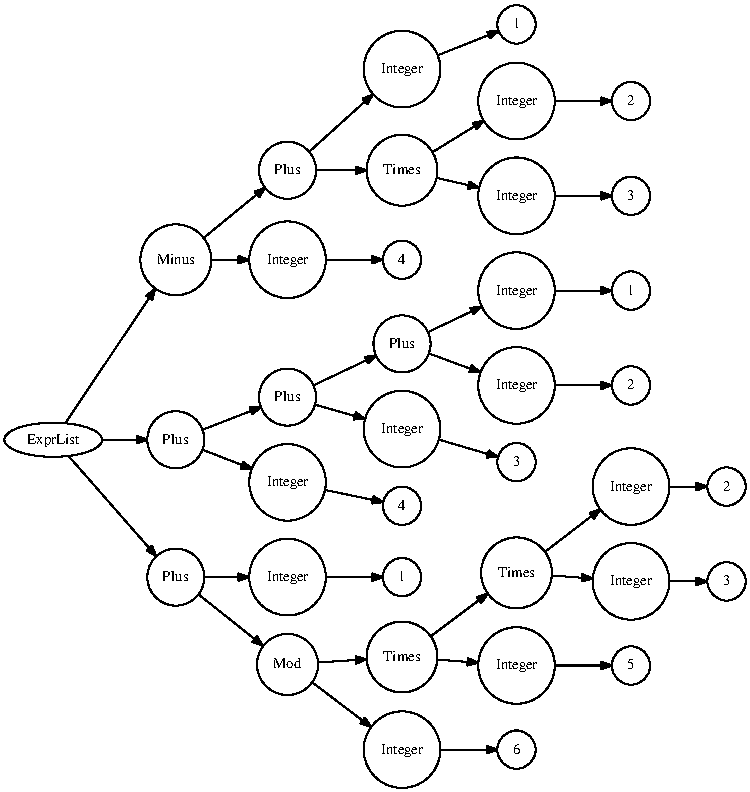
\includegraphics{arith_expr_tree.pdf}
	%\caption{Arithexpr AST}
	%\label{fig:arith_expr_tree}
%\end{figure}

\subsection{Programmiersprachen Parser}
Eine Erweiterung der arithmethischen Ausdrücken um Ausgabe-, sowie Zuweisungsfunktionen spiegelt diese simple Programmiersprache wieder.
Der Scanner \mRefFigure{fig:example_interpreter_grammar_scanner} besteht aus den Tokens für Dezimalzahlen, Variablen, Kommentaren und Leerzeichen o.ä.
\begin{figure}[!htb]
\begin{Verbatim}[ frame         = lines, 
                  framesep      = 0.3cm, 
                  labelposition = bottomline,
                  numbers       = left,
                  numbersep     = -0.2cm,
                  xleftmargin   = 0.8cm,
                  xrightmargin  = 0.8cm,
                ]
  WHITESPACE  := [ \t\v\r\s] ;
  INTEGER     := 0|[1-9][0-9]* ;
  ZID         := [a-zA-Z_][a-zA-Z0-9_]* ;
  SKIP        := {WHITESPACE}|\n|//[^\n]* ;
\end{Verbatim}
\caption{Scannerdefinition für Programmiersprache}
\label{fig:example_interpreter_grammar_scanner}
\end{figure}
Die Anweisungen und Definitionen \mRefFigure{fig:example_interpreter_grammar_statements} beschreiben den Aufbau der Eingabedatei. Sie besteht aus Zuweisungen oder Ausgaben. Diese können wieder aus arithmetischen Ausdrücken bestehen.
\begin{figure}[!htb]

\begin{Verbatim}[ frame         = lines, 
                  framesep      = 0.3cm, 
                  labelposition = bottomline,
                  numbers       = left,
                  numbersep     = -0.2cm,
                  xleftmargin   = 0.8cm,
                  xrightmargin  = 0.8cm,
                ]
  program 
    ::= stmntList:d              {: result := Program(d); :}
    ;
  stmntList
    ::= statement:s stmntList:sl {: result := [s] + sl ; :}
     |                           {: result := []; :}
     ;
  statement 
   ::= ZID:id '=' expr:e ';'     {: result := Assignment(id, e); :}    
     | 'print' '(' expr:e ')' ';'{: result := PrintExpr(e); :}                                 
     ;
  expr 
    ::= expr:e '+'   prod:p      {: result := Sum(e,p); :} 
      | expr:e '-'  prod:p       {: result := Difference(e,p); :} 
      | prod:p                   {: result := p; :}
      ;
  prod 
    ::= prod:p '*'  fact:f       {: result := Product(p,f); :}
      | prod:p '\' fact:f        {: result := Quotient(p,f); :} 
      | fact:f                   {: result := f; :}
      ;
  fact 
    ::= '(' expr:e ')'           {: result := e; :} 
      |  INTEGER:n               {: result := Integer(eval(n)); :} 
      |  ZID:id_1                {: result := Variable(id_1); :}
      ;
\end{Verbatim}
\caption{Grammatik für Progammiersprachenparser}
\label{fig:example_interpreter_grammar_statements}
\end{figure}
Ein Beispiel Programm \mRefFigure{fig:example_interpreter_input} wird durch den Syntaxbaum \mRefFigure{fig:interpreter_tree} abgebildet.
Die Ausgabe des Programms könnte dabei für die Erstellung eines Interpreters genutzt werden.
\begin{figure}[!htb]

\begin{Verbatim}[ frame         = lines, 
                  framesep      = 0.3cm, 
                  labelposition = bottomline,
                  numbers       = left,
                  numbersep     = -0.2cm,
                  xleftmargin   = 0.8cm,
                  xrightmargin  = 0.8cm,
                ]
  a := 5;
  b := 7;
  c := b*a +a\b*(7+6);
  print(c\2);
\end{Verbatim}
\caption{Example interpreter input}
\label{fig:example_interpreter_input}
\end{figure}

\begin{figure}[!htb]
	\centering
		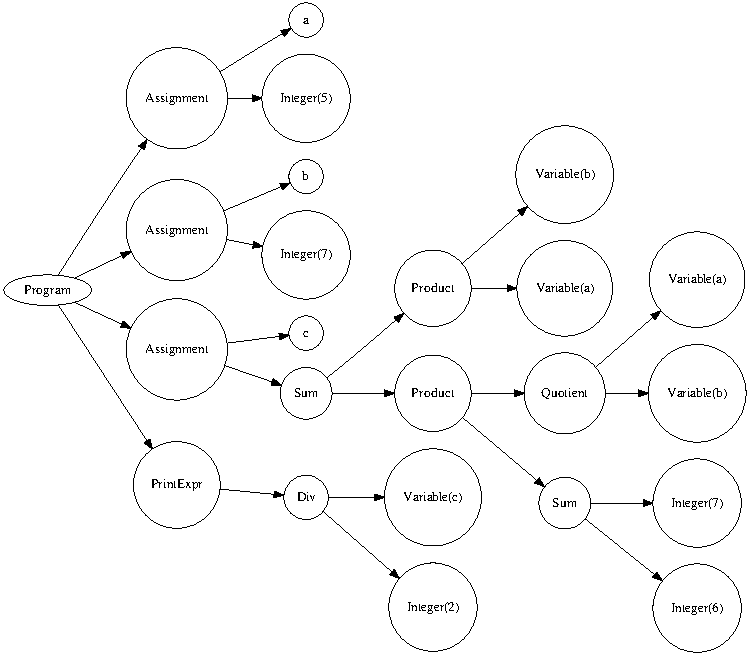
\includegraphics{simple_interpreter_tree.pdf}
	\caption{Interpreter AST}
	\label{fig:interpreter_tree}
\end{figure}

